% =====================================================================
%  Taller Práctico 2 — Infraestructura TI (NRC 8485) — Grupo 6
%  Caso VAR: comparación AWS vs. Azure y propuesta de infraestructura cloud
%  Compilar con:  latexmk -xelatex Entrega2_GRUPO6_NRC8485.tex
%  (xelatex + biber; si no están las fuentes Charter/Avenir Next se usa
%   Latin Modern automáticamente)
% =====================================================================
\documentclass[11pt,letterpaper]{article}

% ---------- Idioma y fuentes ----------
\usepackage{amsmath}
\usepackage{fontspec}
\usepackage[spanish,es-tabla,es-nodecimaldot,es-noshorthands]{babel}
\IfFontExistsTF{Charter}{\setmainfont{Charter}}{\setmainfont{Latin Modern Roman}}
\IfFontExistsTF{Avenir Next}{\setsansfont{Avenir Next}}{\setsansfont{Latin Modern Sans}}
\IfFontExistsTF{Menlo}{\setmonofont[Scale=0.86]{Menlo}}{}

% ---------- Página ----------
\usepackage[letterpaper,top=2.4cm,bottom=2.4cm,left=2.5cm,right=2.5cm,headheight=14pt]{geometry}
\usepackage{fancyhdr}
\usepackage{lastpage}
\usepackage{setspace}
\setstretch{1.08}
\setlength{\parskip}{0.45em}
\setlength{\parindent}{0pt}
\setlength{\emergencystretch}{2em}

% ---------- Tablas, figuras y color ----------
\usepackage[table]{xcolor}
\definecolor{navy}{HTML}{1F3A5F}
\definecolor{ink}{HTML}{22303C}
\definecolor{awsorange}{HTML}{D9822B}
\definecolor{azblue}{HTML}{2B7BB9}
\definecolor{teal}{HTML}{1C7C74}
\definecolor{purple}{HTML}{6B4C9A}
\definecolor{okgreen}{HTML}{CFE8D4}
\definecolor{midamber}{HTML}{FBE3B8}
\definecolor{hired}{HTML}{F4C7C3}
\definecolor{rowgray}{HTML}{F3F5F8}
\usepackage{graphicx}
\usepackage{booktabs}
\usepackage{tabularx}
\usepackage{longtable}
\usepackage{array}
\usepackage{multirow}
\usepackage{makecell}
\usepackage{caption}
\captionsetup{font={small,sf}, labelfont={bf,color=navy}, skip=6pt}
\usepackage{float}
\usepackage{enumitem}
\setlist{itemsep=1pt, topsep=3pt, leftmargin=1.4em}
\usepackage{tikz}
\usetikzlibrary{arrows.meta,positioning,fit,calc}
\usepackage{pgfplots}
\pgfplotsset{compat=1.18}
\usepackage{pgfgantt}
\newcolumntype{Y}{>{\raggedright\arraybackslash}X}
\newcolumntype{R}[1]{>{\raggedleft\arraybackslash}p{#1}}
\newcolumntype{L}[1]{>{\raggedright\arraybackslash}p{#1}}
\renewcommand{\arraystretch}{1.18}

% ---------- Títulos ----------
\usepackage{titlesec}
\titleformat{\section}{\sffamily\Large\bfseries\color{navy}}{\thesection}{0.7em}{}
\titleformat{\subsection}{\sffamily\large\bfseries\color{ink}}{\thesubsection}{0.6em}{}
\titleformat{\subsubsection}{\sffamily\normalsize\bfseries\color{ink}}{\thesubsubsection}{0.5em}{}
\titlespacing*{\section}{0pt}{1.2em}{0.5em}
\titlespacing*{\subsection}{0pt}{0.9em}{0.3em}

% ---------- Bibliografía APA 7 ----------
\usepackage{csquotes}
\usepackage[style=apa,backend=biber]{biblatex}
\addbibresource{referencias.bib}

% ---------- Enlaces ----------
\usepackage{xurl}
\usepackage[hidelinks]{hyperref}
\hypersetup{pdftitle={Taller 2 - Propuesta de infraestructura cloud para VAR - Grupo 6 NRC 8485},
            pdfauthor={Grupo 6: Peña, Morales, Pacheco, Burgos, Muñoz}}

% ---------- Encabezado y pie ----------
\pagestyle{fancy}
\fancyhf{}
\fancyhead[L]{\sffamily\scriptsize\color{ink!70}Infraestructura TI · NRC 8485 · Grupo 6}
\fancyhead[R]{\sffamily\scriptsize\color{ink!70}Taller 2 — Infraestructura cloud para VAR}
\fancyfoot[C]{\sffamily\small Página \thepage\ de \pageref*{LastPage}}
\renewcommand{\headrulewidth}{0.3pt}

% ---------- Atajos ----------
\newcommand{\usd}[1]{US\$\,#1}
\newcommand{\nota}[1]{{\small\color{ink!75}#1}}
\newcommand{\lvl}[1]{%
  \ifnum#1>14 \cellcolor{hired}\textbf{#1}\else
  \ifnum#1>7 \cellcolor{midamber}\textbf{#1}\else
  \cellcolor{okgreen}\textbf{#1}\fi\fi}

\begin{document}

% =====================================================================
%  PORTADA
% =====================================================================
\begin{titlepage}
\thispagestyle{empty}
\centering

\includegraphics[height=3.6cm]{figuras/logo-unab.png}\par
\vspace{0.6cm}
{\sffamily\large Facultad de Ingeniería · Ingeniería Civil Informática\par}
{\sffamily Infraestructura TI · Sección NRC 8485\par}
\vspace{1.6cm}
{\sffamily\color{awsorange}\bfseries\large TALLER PRÁCTICO 2\par}
\vspace{0.3cm}
{\sffamily\bfseries\color{navy}\fontsize{24}{30}\selectfont Infraestructura cloud para VAR:\\[2pt] AWS frente a Azure\par}
\vspace{0.4cm}
{\large Análisis comparativo, estimación de costos, arquitectura\\ y plan de implementación\par}
\vspace{1.4cm}
{\sffamily\bfseries\color{navy} GRUPO 6 — INTEGRANTES Y ROLES\par}
\vspace{0.25cm}
\begin{tabular}{ll}
\toprule
\textbf{Integrante} & \textbf{Rol en el taller}\\
\midrule
Benjamín Peña Díaz & Coordinación, arquitectura y recomendación\\
Francisco Morales Díaz & Investigación de servicios AWS\\
Julián Pacheco Muñoz & Investigación de servicios Azure\\
Martín Burgos Vega & Estimación de costos y calculadoras\\
Matías Muñoz Parraguirre & Migración, riesgos y cumplimiento\\
\bottomrule
\end{tabular}\par
\vfill
{\sffamily Docente: \textbf{Eduardo Correa Marchant}\par}
\vspace{0.2cm}
{\sffamily Santiago, 10 de noviembre de 2026\par}
\end{titlepage}

% =====================================================================
%  ÍNDICES
% =====================================================================
\pagenumbering{roman}
\setcounter{page}{1}
{\hypersetup{linkcolor=ink}\tableofcontents}
\vspace{0.6em}
{\small\listoffigures}
{\small\listoftables}
\clearpage
\pagenumbering{arabic}
\setcounter{page}{1}

% =====================================================================
\section{Introducción y objetivos}
% =====================================================================
VAR es una empresa ficticia con 50 empleados que administra 200 cuentas de clientes y procesa sus transacciones. Su plan de negocio contempla abrir operaciones en cuatro estados adicionales, lo que exige una infraestructura tecnológica \emph{segura, disponible y escalable} para almacenar información y procesar transacciones. La gerencia pidió evaluar Amazon Web Services (AWS) y Microsoft Azure y recomendar una alternativa con criterios técnicos, económicos y regulatorios.

El problema no es solo elegir un proveedor: la infraestructura que se arme hoy tiene que crecer de una a cinco entidades federativas sin rehacerse, cumplir la ley de datos personales del país y tener un costo predecible. Por eso el informe compara los tres pares de servicios que pide el caso (cómputo, almacenamiento de objetos y base de datos administrada), estima su costo en dos escenarios con tarifas oficiales y termina en una arquitectura concreta, con su plan de migración, riesgos, continuidad, cronograma e indicadores.

\textbf{Alcance.} Es un trabajo de investigación: no se crearon recursos en ninguna nube. Todo dato que el caso no entrega se declara como supuesto cuantificable (sección~\ref{sec:supuestos}). Los costos son estimaciones de lista, no cotizaciones comerciales.

\textbf{Objetivo general.} Diseñar y justificar una propuesta de infraestructura cloud para VAR que soporte su operación actual y su expansión a cuatro estados, comparando AWS y Azure con criterios técnicos, económicos, de seguridad y de cumplimiento.

\textbf{Objetivos específicos} (alineados con los resultados de aprendizaje RA1–RA5):
\begin{enumerate}
  \item Investigar en documentación oficial las capacidades y limitaciones de Amazon EC2, Amazon S3, Amazon RDS, Azure Virtual Machines, Azure Blob Storage y Azure SQL Database (RA1).
  \item Comparar los tres pares de servicios con criterios verificables aplicados a VAR (RA2).
  \item Estimar el costo mensual y anual de ambos proveedores en un escenario actual y otro de expansión, con región, moneda, fecha y fórmulas explícitas (RA3).
  \item Proponer una arquitectura y un plan de implementación con migración, riesgos, continuidad, cronograma, KPI y cumplimiento normativo (RA4).
  \item Comunicar la propuesta en este informe y en una defensa oral de diez minutos (RA5).
\end{enumerate}

% =====================================================================
\section{Supuestos de trabajo}\label{sec:supuestos}
% =====================================================================
El caso no especifica país, estados, volumen de datos, infraestructura actual ni presupuesto. La tabla~\ref{tab:supuestos} declara los supuestos mínimos que pide el enunciado y la tabla~\ref{tab:supuestos2} los complementarios que usa el resto del informe. Ninguno es un hecho del caso: son decisiones del grupo, cuantificadas y usadas de forma consistente en todas las secciones.

\begin{table}[H]
\centering\small
\caption{Supuestos mínimos del caso VAR (sección 4 del enunciado).}\label{tab:supuestos}
\begin{tabularx}{\linewidth}{L{2.3cm}YY}
\toprule
\textbf{Supuesto} & \textbf{Hoy} & \textbf{Tras la expansión (mes 24)}\\
\midrule
Territorio & México. Opera en la Ciudad de México (matriz). & Se suman \textbf{Nuevo León, Jalisco, Querétaro y Puebla}: cinco entidades en total.\\
\rowcolor{rowgray} Usuarios & 50 internos; 300 externos (200 cuentas × 1,5 usuarios). Concurrencia en hora punta: \textbf{95} (70\,\% de internos y 20\,\% de externos). & 110 internos (15 por estado nuevo); 900 externos (600 cuentas). Concurrencia en hora punta: \textbf{260}.\\
Datos & \textbf{0,45 TB}: base de datos de 40 GB y 400 GB de documentos (PDF y XML de facturas y contratos). & \textbf{2 TB}: base de datos de 150 GB y 1,8 TB de documentos.\\
\rowcolor{rowgray} Transacciones & \textbf{60.000 al mes} (≈ 300 por cuenta), con 20\,\% concentrado en los 3 días de cierre. & \textbf{200.000 al mes}, más un crecimiento orgánico del 15\,\% anual.\\
Disponibilidad & \multicolumn{2}{>{\raggedright\arraybackslash}p{\dimexpr\linewidth-2.3cm-4\tabcolsep\relax}}{\textbf{99,9\,\% mensual} del servicio transaccional (como máximo 43,8 minutos de caída al mes).}\\
\rowcolor{rowgray} Continuidad & \multicolumn{2}{>{\raggedright\arraybackslash}p{\dimexpr\linewidth-2.3cm-4\tabcolsep\relax}}{\textbf{RPO 15 minutos y RTO 4 horas} ante fallas de instancia, de zona o de datos. Ante un desastre que afecte a toda la región: RPO 24 h y RTO 24 h, aceptado por la gerencia.}\\
\bottomrule
\end{tabularx}
\end{table}

\begin{table}[H]
\centering\small
\caption{Supuestos complementarios usados en el diseño y en los costos.}\label{tab:supuestos2}
\begin{tabularx}{\linewidth}{L{3.4cm}Y}
\toprule
\textbf{Supuesto} & \textbf{Valor declarado}\\
\midrule
Rubro de VAR & Servicios de administración y cobranza para pymes: emite facturas electrónicas (CFDI) y registra pagos de sus clientes. No almacena datos de tarjetas: los cobros pasan por una pasarela externa, así que PCI DSS queda fuera del alcance.\\
\rowcolor{rowgray} Infraestructura actual & Sala de servidores en la oficina de la CDMX: un servidor Linux con la aplicación web, PostgreSQL 14 y un NAS de 400 GB. Equipos con más de cinco años de uso y sin respaldo fuera del edificio.\\
Aplicación & Aplicación web propia (portal de clientes y backoffice) sobre PostgreSQL, sin estado en el servidor, que puede escalar horizontalmente.\\
\rowcolor{rowgray} Equipo de TI & Dos personas (líder de TI y analista), con apoyo de un partner externo durante la migración.\\
Identidad y licencias & Correo y cuentas en Google Workspace. VAR no tiene contrato empresarial con Microsoft ni licencias de Windows Server o SQL Server con Software Assurance.\\
\rowcolor{rowgray} Tráfico y solicitudes & Salida a Internet de 150 GB al mes hoy y 600 GB en la expansión. Objetos: 200.000 escrituras y 2 millones de lecturas al mes hoy (×4 en la expansión).\\
Presupuesto & Techo de \usd{15.000} al año para la infraestructura cloud en la expansión, sin impuestos.\\
\bottomrule
\end{tabularx}
\end{table}

% =====================================================================
\section{Investigación de servicios}\label{sec:investigacion}
% =====================================================================
Los seis servicios son ofertas de \emph{infraestructura como servicio} (IaaS: EC2 y Azure VM) o de \emph{plataforma como servicio} (PaaS: S3, Blob Storage, RDS y Azure SQL Database), según la definición de \textcite{nist800145}. La diferencia importa porque cambia qué parte de la seguridad y de la operación queda en manos de VAR: en IaaS VAR administra el sistema operativo, los parches y la aplicación; en PaaS el proveedor opera el motor y el hardware, y VAR responde por los datos, las identidades y la configuración \parencite{aws-shared,az-shared}.

\subsection{Cómputo: Amazon EC2 y Azure Virtual Machines}
\textbf{Capacidades.} Ambos entregan máquinas virtuales bajo demanda, con cientos de tamaños agrupados en familias (uso general, cómputo, memoria, almacenamiento y GPU), Linux o Windows, discos en bloque persistentes (EBS en AWS y Managed Disks en Azure) y redes virtuales privadas \parencite{aws-ec2,az-vm}. Para VAR se comparan dos tamaños equivalentes de uso general con 2 vCPU y 8 GiB: \texttt{m7i.large} en AWS y \texttt{D2s v5} en Azure \parencite{aws-ec2-types,az-dsv5}.

\textbf{Limitaciones.} Cada cuenta o suscripción tiene una cuota de vCPU por región y por familia que hay que ampliar con una solicitud antes de crecer. Las regiones nuevas, como las de México, no ofrecen todas las familias de instancias. La disponibilidad comprometida depende de cómo se despliegue: una instancia sola tiene un SLA menor que varias repartidas en zonas de disponibilidad. AWS publica 99,99\,\% para instancias en dos o más zonas y 99,5\,\% para una instancia individual \parencite{aws-sla-compute}; Azure publica 99,99\,\% para VM en dos o más zonas y 99,9\,\% para una VM sola con discos Premium SSD \parencite{az-sla}.

\textbf{Escalabilidad.} El escalado vertical (cambiar de tamaño) exige reiniciar la máquina. El horizontal se automatiza con EC2 Auto Scaling y con Virtual Machine Scale Sets, que agregan o quitan instancias según la carga y las reparten entre zonas \parencite{aws-asg,az-vmss}.

\textbf{Ajuste a VAR.} El portal y el backoffice corren en dos instancias, una por zona, detrás de un balanceador. Con 95 usuarios concurrentes hoy y 260 en la expansión, el patrón horizontal (de 2 a 4–6 instancias) cubre el crecimiento sin rediseñar nada, y la redundancia entre zonas sostiene el 99,9\,\% comprometido.

\subsection{Almacenamiento de objetos: Amazon S3 y Azure Blob Storage}
\textbf{Capacidades.} Ambos guardan objetos (archivos con metadatos) en contenedores sin límite práctico de capacidad, con clases o niveles de acceso que bajan el costo de los datos poco consultados, versionado, ciclo de vida, cifrado en reposo por defecto e inmutabilidad (WORM) para cumplimiento \parencite{aws-s3,aws-s3-lock,az-blob}. S3 Standard replica los objetos en al menos tres zonas de disponibilidad; en Azure el equivalente es la redundancia de zona (ZRS), porque la opción local (LRS) mantiene las tres copias en un solo centro de datos \parencite{az-redundancy}.

\textbf{Limitaciones.} S3 sostiene al menos 3.500 escrituras y 5.500 lecturas por segundo por prefijo \parencite{aws-s3-perf}. Una cuenta estándar de Azure Storage tiene un tope por defecto de 5 PiB y una tasa máxima de solicitudes por cuenta \parencite{az-blob-scale}. Ninguno es un sistema de archivos POSIX, así que la aplicación accede por API o SDK. El SLA publicado para el nivel caliente es de 99,9\,\% en ambos \parencite{aws-sla-s3,az-sla}.

\textbf{Ajuste a VAR.} Aquí viven los PDF y XML de facturas y contratos (de 400 GB hoy a 1,8 TB después). El versionado y el bloqueo de objetos protegen contra borrados y ransomware, y el ciclo de vida mueve a almacenamiento de archivo lo que tiene más de un año, conservándolo los cinco años que exige la ley fiscal (sección~\ref{sec:cumplimiento}).

\subsection{Base de datos administrada: Amazon RDS y Azure SQL Database}
\textbf{Capacidades.} Amazon RDS administra seis motores (PostgreSQL, MySQL, MariaDB, Oracle, SQL Server y Db2): aprovisiona, parcha, respalda y conmuta por error, y ofrece Multi-AZ con una réplica síncrona en otra zona \parencite{aws-rds,aws-rds-maz}. Azure SQL Database es un servicio administrado del motor SQL Server; ofrece los niveles General Purpose, Business Critical y Hyperscale, y llega hasta 128 vCore y 4 TB, o hasta 128 TB en Hyperscale \parencite{az-sqldb}.

\textbf{Equivalencia.} RDS no tiene un único par en Azure: el equivalente depende del motor. Como VAR usa PostgreSQL (tabla~\ref{tab:supuestos2}), el par justo es \emph{RDS for PostgreSQL} frente a \emph{Azure Database for PostgreSQL – Flexible Server}, como permite el enunciado \parencite{az-pg}. Azure SQL Database solo sería la opción natural si VAR usara SQL Server, porque obligaría a migrar el motor y a reescribir consultas y procedimientos.

\textbf{Limitaciones y disponibilidad.} RDS no da acceso al sistema operativo ni a superusuario, admite hasta 15 réplicas de lectura por instancia primaria y retiene respaldos automáticos entre 1 y 35 días con recuperación a un punto en el tiempo (PITR) \parencite{aws-rds-limits,aws-rds-backup}. Su SLA para Multi-AZ es de 99,95\,\% \parencite{aws-sla-rds}. PostgreSQL Flexible Server admite hasta cinco réplicas de lectura, retiene respaldos de 7 a 35 días y, con alta disponibilidad con redundancia de zona, publica un SLA de 99,99\,\% \parencite{az-pg-replicas,az-pg-backup,az-pg-ha}. Una limitación pesa para VAR: el respaldo geo-redundante de Flexible Server solo funciona en regiones con par asignado, y \emph{Mexico Central no tiene par} \parencite{az-pg-backup,az-pairs}.

\textbf{Ajuste a VAR.} Las 60.000 transacciones al mes de hoy, que serán 200.000, son una carga baja para una instancia de 2 vCPU (menos de una transacción por segundo incluso en los días de cierre). Lo que manda el tamaño es la disponibilidad, no el rendimiento, y por eso ambos lados usan una réplica síncrona en otra zona.

\subsection{Matriz comparativa 1: servicios y ajuste funcional}
La tabla~\ref{tab:matriz1} resume la investigación. El costo mensual corresponde al escenario actual de la sección~\ref{sec:costos}.

\begin{table}[tbp]
\centering\footnotesize
\caption{Matriz comparativa 1: servicios y ajuste funcional para VAR.}\label{tab:matriz1}
\begin{tabularx}{\linewidth}{L{2.35cm}YY}
\toprule
\textbf{Criterio} & \textbf{AWS (EC2 / S3 / RDS)} & \textbf{Azure (VM / Blob / SQL DB)}\\
\midrule
Servicio y función & EC2: VM IaaS. S3: objetos PaaS. RDS: base relacional administrada con seis motores. & VM: IaaS. Blob: objetos PaaS. SQL Database: SQL Server administrado; para PostgreSQL, Flexible Server.\\
\rowcolor{rowgray} Capacidades y limitaciones & Cuotas de vCPU por región. S3: 3.500/5.500 sol./s por prefijo. RDS: hasta 15 réplicas, PITR de 1 a 35 días, sin acceso al SO. & Cuotas de vCPU por familia. Blob: 5 PiB por cuenta por defecto. SQL DB: hasta 4 TB (128 TB en Hyperscale). PostgreSQL: 5 réplicas, PITR de 7 a 35 días, sin geo-respaldo en Mexico Central.\\
Aplicación concreta en VAR & 2 × \texttt{m7i.large} (4 en la expansión), S3 para facturas y contratos, RDS PostgreSQL Multi-AZ \texttt{db.m7g.large} (\texttt{xlarge} en la expansión). & 2 × \texttt{D2s v5} (4 en la expansión), Blob caliente ZRS, PostgreSQL Flexible GP de 2 vCore (4 en la expansión) con HA de zona.\\
\rowcolor{rowgray} Escalabilidad y rendimiento & Auto Scaling horizontal en 3 zonas; RDS escala de forma vertical y con réplicas de lectura. & Scale Sets en 3 zonas; Flexible Server escala de forma vertical y con réplicas; SQL DB, además, con Hyperscale y serverless.\\
Seguridad, respaldo y SLA publicado & KMS, IAM, cifrado por defecto en S3. SLA: EC2 en 2+ zonas 99,99\,\%; S3 99,9\,\%; RDS Multi-AZ 99,95\,\%. Copia de respaldos entre regiones con AWS Backup. & Key Vault, Entra ID y cifrado por defecto. SLA: VM en zonas 99,99\,\%; Blob caliente 99,9\,\%; PostgreSQL con HA de zona 99,99\,\%. Sin par regional para el geo-respaldo.\\
\rowcolor{rowgray} Costo mensual estimado (actual) & \textbf{\usd{495,45}} & \textbf{\usd{564,73}}\\
\bottomrule
\end{tabularx}
\end{table}

% =====================================================================
\section{Estimación de costos}\label{sec:costos}
% =====================================================================
\subsection{Metodología}
\begin{itemize}
  \item \textbf{Regiones:} AWS \texttt{mx-central-1} (México Central, Querétaro) y Azure \emph{Mexico Central} (Querétaro). Se eligieron porque dejan los datos en el país y a pocos milisegundos de las cinco entidades \parencite{aws-regions,az-geos}.
  \item \textbf{Moneda y fecha:} dólares estadounidenses (USD), sin impuestos (el IVA en México es de 16\,\%). Tarifas consultadas el \textbf{10 de noviembre de 2026}.
  \item \textbf{Fuente:} \textbf{AWS Pricing Calculator} y \textbf{Azure Pricing Calculator}, configuradas sin iniciar sesión, cuyas tarifas coinciden con las de las interfaces oficiales que las alimentan: AWS Price List Bulk API (archivos de \texttt{mx-central-1} del 29 de octubre al 9 de noviembre de 2026) y Azure Retail Prices API \parencite{aws-calc,az-calc,aws-pricelist,az-retail}. Enlaces y capturas en el Anexo~\ref{anx:calculadoras}.
  \item \textbf{Modalidad de cobro:} pago por uso (On-Demand), sin compromisos ni descuentos. No se usan capas gratuitas: Azure Pricing Calculator descuenta los primeros 100 GB de salida y el grupo los suma de vuelta (\usd{8,70} al mes). El efecto de reservar por un año se muestra aparte, como sensibilidad.
  \item \textbf{Fórmulas:} un mes tiene 730 horas. Para cada línea, \(\text{Costo} = \text{Cantidad} \times \text{Tarifa}\); el total mensual es la suma de las líneas y el total anual es igual a \(12 \times\) el total mensual. El detalle de cada línea está en el Anexo~\ref{anx:detalle} y en la planilla Excel que acompaña al informe.
\end{itemize}

\subsection{Configuración elegida}
Para que la comparación sea justa se configuró la misma arquitectura en ambos proveedores: dos servidores de aplicación en zonas distintas, almacenamiento de objetos redundante entre zonas y una base PostgreSQL con réplica síncrona en otra zona (tabla~\ref{tab:config}).

\begin{table}[H]
\centering\footnotesize
\caption{Configuración dimensionada por escenario.}\label{tab:config}
\begin{tabularx}{\linewidth}{L{2.6cm}YY}
\toprule
\textbf{Componente} & \textbf{Escenario actual} & \textbf{Escenario de expansión}\\
\midrule
Cómputo & 2 VM de 2 vCPU y 8 GiB, con disco de 64 GB cada una & 4 VM de 2 vCPU y 8 GiB (promedio del Auto Scaling)\\
\rowcolor{rowgray} Objetos & 500 GB; 0,2 M escrituras y 2 M lecturas al mes & 2.000 GB; 0,8 M escrituras y 8 M lecturas al mes\\
Base de datos & PostgreSQL de 2 vCPU y 8 GiB con réplica en otra zona; 128 GB & PostgreSQL de 4 vCPU y 16 GiB con réplica en otra zona; 256 GB\\
\rowcolor{rowgray} Respaldos & 64 GB de respaldo de la base sobre lo incluido; snapshot diario de cada VM (1 GB de cambio al día) & 128 GB de respaldo de la base; snapshot diario de las 4 VM\\
Transferencia & 150 GB de salida a Internet al mes & 600 GB de salida a Internet al mes\\
\bottomrule
\end{tabularx}
\end{table}

\subsection{Matriz comparativa 2: escenario actual}
\begin{table}[H]
\centering\footnotesize
\caption{Matriz comparativa 2, escenario actual (USD/mes, 10-11-2026). Estimaciones en el Anexo~\ref{anx:calculadoras}.}\label{tab:m2a}
\begin{tabularx}{\linewidth}{L{3.2cm}R{1.55cm}R{1.55cm}Y}
\toprule
\textbf{Concepto} & \textbf{AWS} & \textbf{Azure} & \textbf{Supuesto / fuente (región, cantidad y tarifa)}\\
\midrule
Cómputo (VM) & 165,28 & 177,22 & 2 × 730 h. AWS: \texttt{m7i.large} a 0,10584/h más EBS gp3 a 0,084/GB-mes. Azure: \texttt{D2s v5} a 0,106/h más P6 a 11,23/disco-mes.\\
\rowcolor{rowgray} Almacenamiento de objetos & 13,97 & 16,56 & 500 GB. S3 Standard a 0,02415/GB; Blob caliente ZRS a 0,0286/GB; más solicitudes.\\
Base de datos administrada & 287,94 & 318,25 & RDS \texttt{db.m7g.large} Multi-AZ a 0,352/h más 128 GB a 0,242. Flexible GP 2 vCore × 2 (HA) a 0,0979/vCore-h más 128 GB × 2 a 0,1265.\\
\rowcolor{rowgray} Backups y snapshots & 14,77 & 39,66 & AWS: 64 GB × 0,10 más snapshots diarios de EBS, 158 GB-mes × 0,053. Azure: 64 GB × 2 (HA) × 0,1045, 2 VM protegidas × 11,00, 166,4 GB × 0,02464 y 1,28 GB × 0,145.\\
Transferencia de datos & 13,50 & 13,05 & 150 GB de salida. AWS 0,09/GB; Azure 0,087/GB.\\
\midrule
\textbf{TOTAL mensual} & \textbf{495,45} & \textbf{564,73} & Azure, +14,0\,\%. Calculadoras: 495,45 y 556,03 + 8,70.\\
\textbf{TOTAL anual} & \textbf{5.945,40} & \textbf{6.776,76} & \(12 \times\) total mensual. Costo por cuenta: \usd{2,48} (AWS) y \usd{2,82} (Azure) al mes.\\
\bottomrule
\end{tabularx}
\end{table}

\subsection{Matriz comparativa 2: escenario de expansión a cuatro estados}
\begin{table}[H]
\centering\footnotesize
\caption{Matriz comparativa 2, escenario de expansión (USD/mes, 10-11-2026). Estimaciones en el Anexo~\ref{anx:calculadoras}.}\label{tab:m2b}
\begin{tabularx}{\linewidth}{L{3.2cm}R{1.55cm}R{1.55cm}Y}
\toprule
\textbf{Concepto} & \textbf{AWS} & \textbf{Azure} & \textbf{Supuesto / fuente (región, cantidad y tarifa)}\\
\midrule
Cómputo (VM) & 330,56 & 354,43 & 4 × 730 h, con las mismas tarifas del escenario actual.\\
\rowcolor{rowgray} Almacenamiento de objetos & 55,86 & 66,22 & 2.000 GB, 0,8 M escrituras y 8 M lecturas.\\
Base de datos administrada & 575,87 & 636,50 & RDS \texttt{db.m7g.xlarge} Multi-AZ a 0,704/h más 256 GB. Flexible GP 4 vCore × 2 (HA) más 256 GB × 2.\\
\rowcolor{rowgray} Backups y snapshots & 29,55 & 79,32 & AWS: 128 GB de respaldo de la base y 316 GB-mes de snapshots. Azure: 128 GB × 2 (HA), 4 VM protegidas × 11,00, 332,8 GB y 2,56 GB.\\
Transferencia de datos & 54,00 & 52,20 & 600 GB de salida.\\
\midrule
\textbf{TOTAL mensual} & \textbf{1.045,84} & \textbf{1.188,68} & Azure, +13,7\,\%. Calculadoras: 1.045,83 y 1.179,98 + 8,70.\\
\textbf{TOTAL anual} & \textbf{12.550,08} & \textbf{14.264,16} & Ambos bajo el techo de \usd{15.000} al año. Costo por cuenta: \usd{1,74} y \usd{1,98} al mes.\\
\bottomrule
\end{tabularx}
\end{table}

\subsection{Costos omitidos y sensibilidad}
Las matrices cubren las cinco categorías que pide el enunciado. Quedan fuera, en ambos proveedores, el balanceador de carga y el firewall de aplicaciones (en AWS el ALB parte en 0,0236 USD/h, unos \usd{17} al mes más capacidad), la VPN de la migración, las IP públicas, el monitoreo y los registros, el servicio de claves, el plan de soporte, la copia de respaldos en una segunda región y el IVA. Como supuesto, el grupo estima que estos elementos suman entre 20\,\% y 30\,\% sobre el total; aun así, el escenario de expansión en AWS (\(12.550 \times 1{,}3 \approx\) \usd{16.300}) quedaría cerca del techo de presupuesto, que habría que revisar.

\begin{figure}[H]
\centering
% Gráfico de costos mensuales por escenario. Se incluye con \input.
\begin{tikzpicture}
\begin{axis}[
  ybar, bar width=15pt, width=0.96\linewidth, height=6.2cm,
  ymin=0, ymax=1400, ylabel={USD por mes}, ylabel style={font=\sffamily\small},
  symbolic x coords={A,B,C,D},
  xticklabels={{Actual\\pago por uso},{Expansión\\pago por uso},{Actual\\reserva 1 año},{Expansión\\reserva 1 año}},
  xtick=data, xticklabel style={align=center, font=\sffamily\small},
  yticklabel style={font=\sffamily\small, /pgf/number format/.cd, 1000 sep={.}},
  nodes near coords, every node near coord/.append style={font=\sffamily\scriptsize, /pgf/number format/.cd, fixed, precision=0, 1000 sep={.}},
  legend style={at={(0.02,0.97)}, anchor=north west, font=\sffamily\small, draw=none},
  legend cell align=left, axis lines*=left, ymajorgrids, grid style={ink!15},
  enlarge x limits=0.18,
]
\addplot[fill=awsorange, draw=awsorange!80!black] coordinates {(A,489.20) (B,1033.33) (C,377.76) (D,810.45)};
\addplot[fill=azblue, draw=azblue!80!black] coordinates {(A,554.75) (B,1168.70) (C,380.96) (D,821.11)};
\legend{AWS (mx-central-1), Azure (Mexico Central)}
\end{axis}
\end{tikzpicture}

\caption{Costo mensual por escenario y modalidad de cobro (USD, 10-11-2026).}\label{fig:costos}
\end{figure}

\textbf{Sensibilidad.} Si VAR se compromete por un año con el cómputo y la base de datos (AWS Reserved Instances sin pago inicial y Azure Reservations), la diferencia casi desaparece: \usd{384,01} frente a \usd{390,94} en el escenario actual y \usd{822,96} frente a \usd{841,09} en la expansión (figura~\ref{fig:costos}). Azure descuenta más al reservar (entre 38\,\% y 40\,\%, contra 23\,\% a 34\,\% en AWS). Por eso el costo por sí solo no decide la recomendación: a mediano plazo pesan más la continuidad y el ajuste operativo (sección~\ref{sec:recomendacion}).

% =====================================================================
\section{Arquitectura y recomendación}\label{sec:recomendacion}
% =====================================================================
\subsection{Matriz de decisión}
Se ponderaron cinco criterios que se desprenden del caso. El puntaje va de 1 a 5 y cada uno se justifica con un dato de las secciones anteriores (tabla~\ref{tab:decision}).

\begin{table}[H]
\centering\footnotesize
\caption{Matriz de decisión ponderada.}\label{tab:decision}
\begin{tabularx}{\linewidth}{L{3.1cm}c cc Y}
\toprule
\textbf{Criterio} & \textbf{Peso} & \textbf{AWS} & \textbf{Azure} & \textbf{Evidencia}\\
\midrule
Seguridad & 25\,\% & 5 & 5 & Cifrado por defecto, claves propias, MFA y servicios de detección equivalentes en ambos.\\
\rowcolor{rowgray} Costo & 25\,\% & 5 & 4 & AWS cuesta 12--14\,\% menos pagando por uso; con reservas la diferencia baja a 2\,\%.\\
Rendimiento y disponibilidad & 20\,\% & 4 & 5 & SLA de la base: 99,95\,\% en RDS Multi-AZ y 99,99\,\% en Flexible Server con HA de zona.\\
\rowcolor{rowgray} Crecimiento & 15\,\% & 5 & 4 & 3 zonas en ambas regiones; 15 réplicas de lectura en RDS y 5 en Flexible Server.\\
Continuidad ante desastre regional & 15\,\% & 5 & 3 & AWS Backup copia a otra región; Mexico Central no tiene par para el geo-respaldo de PostgreSQL.\\
\midrule
\textbf{Puntaje ponderado} & & \textbf{4,80} & \textbf{4,30} & \\
\bottomrule
\end{tabularx}
\end{table}

\subsection{Recomendación}
Se recomienda \textbf{AWS en la región México Central (\texttt{mx-central-1}) como proveedor único}, con la arquitectura de la figura~\ref{fig:arquitectura}. No se propone una arquitectura combinada: con dos personas en TI, operar dos nubes duplica identidades, monitoreo y competencias sin un beneficio claro, y la transferencia entre proveedores agrega costo y latencia.

\begin{figure}[tbp]
\centering
\resizebox{\linewidth}{!}{% Diagrama de arquitectura propuesta (AWS, mx-central-1). Se incluye con \input.
\begin{tikzpicture}[
  font=\sffamily\scriptsize, >=Stealth,
  box/.style={draw=#1, fill=#1!8, rounded corners=2pt, align=center, inner sep=3pt},
  box/.default=navy,
  svc/.style={draw=awsorange, fill=awsorange!10, rounded corners=2pt, align=center, minimum width=2.9cm, minimum height=0.85cm, inner sep=2pt},
  user/.style={draw=ink!70, fill=white, rounded corners=6pt, align=center, minimum width=2.9cm, minimum height=1.1cm},
  lnk/.style={->, thick, draw=ink!75},
  dlnk/.style={->, thick, dashed, draw=ink!55},
  lbl/.style={font=\sffamily\tiny, fill=white, inner sep=1pt}
]
% ---------- Región ----------
\draw[awsorange, very thick, rounded corners=4pt] (6.3,-0.9) rectangle (19.2,8.1);
\node[anchor=north west, font=\sffamily\footnotesize\bfseries, text=awsorange] at (6.4,8.05) {AWS · Región México (Central) \texttt{mx-central-1} · Querétaro};
% ---------- VPC ----------
\draw[navy, thick, rounded corners=3pt] (6.6,-0.6) rectangle (15.3,7.45);
\node[anchor=north west, font=\sffamily\scriptsize\bfseries, text=navy] at (6.7,7.42) {VPC 10.20.0.0/16};
% AZ columns
\foreach \x/\n/\s in {6.85/a/solid, 9.65/b/solid, 12.45/c/dashed}{
  \draw[ink!45, \s, rounded corners=2pt] (\x,-0.4) rectangle ++(2.65,7.4);
  \node[font=\sffamily\tiny\bfseries, text=ink!70] at (\x+1.325,6.8) {Zona de disponibilidad \n};
}
\node[font=\sffamily\tiny, text=ink!60, align=center] at (13.775,6.45) {(se habilita en\\la expansión)};
% row labels
\node[rotate=90, font=\sffamily\tiny, text=ink!60] at (6.72,6.25) {Subred pública};
\node[rotate=90, font=\sffamily\tiny, text=ink!60] at (6.72,3.3) {Subred app};
\node[rotate=90, font=\sffamily\tiny, text=ink!60] at (6.72,-0.05) {Subred datos};
% ALB
\node[box=navy, minimum width=5.2cm, minimum height=0.8cm] (alb) at (9.6,5.4) {\textbf{Application Load Balancer} + AWS WAF\\ TLS 1.2+, certificados ACM};
\node[box=ink, minimum width=2.2cm, minimum height=0.8cm, dashed] (albc) at (13.775,5.4) {nodo ALB};
% EC2
\node[box=teal, minimum width=2.3cm, minimum height=1.05cm] (ec2a) at (8.175,3.3) {EC2 m7i.large\\ aplicación web/API};
\node[box=teal, minimum width=2.3cm, minimum height=1.05cm] (ec2b) at (10.975,3.3) {EC2 m7i.large\\ aplicación web/API};
\node[box=teal, minimum width=2.3cm, minimum height=1.05cm, dashed] (ec2c) at (13.775,3.3) {EC2 adicionales\\ (de 2 a 4–6)};
\draw[teal, densely dotted, thick, rounded corners=3pt] (7.0,2.6) rectangle (14.95,4.0);
% RDS
\node[box=purple, minimum width=2.3cm, minimum height=1.05cm] (rdsa) at (8.175,0.9) {RDS PostgreSQL\\ \textbf{primaria}};
\node[box=purple, minimum width=2.3cm, minimum height=1.05cm] (rdsb) at (10.975,0.9) {RDS PostgreSQL\\ \textbf{standby}};
\node[box=purple, minimum width=2.3cm, minimum height=1.05cm, dashed] (rdsc) at (13.775,0.9) {réplica de lectura\\ (reportería)};
\draw[<->, thick, purple] (rdsa) -- (rdsb);
\node[lbl, text=purple] at (9.575,0.12) {síncrona};
\draw[->, thick, dashed, purple] (rdsb.south) to[bend right=25] node[lbl, below]{asíncrona} (rdsc.south);
% conexiones internas
\draw[lnk] (alb.south) ++(-1.4,0) -- (ec2a.north);
\draw[lnk] (alb.south) ++(1.4,0) -- (ec2b.north);
\draw[lnk] (ec2a.south) -- (rdsa.north);
\draw[lnk] (ec2b.south) -- (rdsa.north east);
% ---------- servicios regionales ----------
\node[svc] (s3)  at (17.25,6.55) {\textbf{Amazon S3}\\ documentos, versionado,\\ Object Lock};
\node[svc] (kms) at (17.25,5.2) {\textbf{AWS KMS}\\ claves gestionadas por VAR};
\node[svc] (bk)  at (17.25,3.95) {\textbf{AWS Backup}\\ planes diarios + PITR};
\node[svc] (obs) at (17.25,2.7) {\textbf{CloudWatch, CloudTrail}\\ GuardDuty, Security Hub};
\node[svc] (idc) at (17.25,1.45) {\textbf{IAM Identity Center}\\ SSO + MFA, roles mínimos};
\node[svc] (ssm) at (17.25,0.2) {\textbf{Systems Manager}\\ acceso admin sin SSH};
\draw[lnk] (14.95,3.3) -- (15.48,3.3) |- node[lbl, rotate=90, pos=0.3]{endpoint privado} (s3.west);
% ---------- usuarios ----------
\node[user] (emp) at (1.6,6.2) {\textbf{Empleados}\\ de 50 a 110, en 5 estados};
\node[user] (cli) at (1.6,4.2) {\textbf{Clientes}\\ de 200 a 600 cuentas};
\node[box=ink, minimum width=2.9cm, minimum height=1.1cm, dashed] (onp) at (1.6,1.0) {\textbf{Centro de datos actual}\\ oficina CDMX\\ (se retira tras el corte)};
\node[box=navy, minimum width=2.4cm, minimum height=0.9cm] (dns) at (4.6,5.2) {Route 53\\ (DNS, TTL 60 s)};
\draw[lnk] (emp.east) -- (dns.north west);
\node[lbl] at (3.55,6.45) {HTTPS + SSO};
\draw[lnk] (cli.east) -- (dns.south west);
\node[lbl] at (3.55,3.95) {HTTPS};
\draw[lnk] (dns.east) -- (alb.west);
\draw[dlnk] (onp.east) -- node[lbl, above, pos=0.42]{VPN sitio a sitio} node[lbl, below, pos=0.42]{DMS + DataSync} (rdsa.west);
% ---------- región secundaria ----------
\draw[ink!60, dashed, rounded corners=3pt] (6.3,-2.5) rectangle (19.2,-1.25);
\node[anchor=west, font=\sffamily\scriptsize, text=ink] at (6.45,-1.875) {\textbf{Región secundaria (EE.\,UU. Este, Ohio)}: copia diaria cifrada de los respaldos para un desastre regional};
\draw[dlnk] (bk.east) -- (18.95,3.95) -- (18.95,-1.25);
\node[font=\sffamily\tiny, text=teal, fill=white, inner sep=1pt] at (11.0,4.0) {EC2 Auto Scaling group (mín. 2, deseado 2 hoy / 4 en expansión)};
\end{tikzpicture}
}
\caption{Arquitectura propuesta para VAR en AWS. Las líneas punteadas son componentes de la expansión o de la migración.}\label{fig:arquitectura}
\end{figure}

\textbf{Cómo funciona.} Empleados y clientes entran por HTTPS a un único dominio (Route 53) que apunta a un Application Load Balancer protegido por AWS WAF. El balanceador reparte la carga entre las instancias EC2 del grupo de Auto Scaling, una por zona, en subredes privadas sin IP pública. La aplicación usa RDS for PostgreSQL Multi-AZ, con la primaria en una zona y la réplica síncrona en otra, y guarda los documentos en S3 mediante un endpoint privado. La administración se hace con Systems Manager, sin abrir SSH, y las identidades se federan desde Google Workspace hacia IAM Identity Center con MFA obligatorio. En la expansión se habilita la tercera zona, el grupo de Auto Scaling crece a 4–6 instancias y se agrega una réplica de lectura para los reportes de las sucursales.

\textbf{Justificación por criterio.}
\begin{itemize}
  \item \textbf{Seguridad:} todo cifrado con claves de KMS que controla VAR, sin servidores expuestos a Internet, con mínimo privilegio y detección continua (GuardDuty y Security Hub), siguiendo el pilar de seguridad del Well-Architected Framework \parencite{aws-waf}.
  \item \textbf{Costo:} es la opción más barata pagando por uso en los dos escenarios (\usd{5.945} y \usd{12.550} al año) y su costo por cuenta baja de \usd{2,48} a \usd{1,74} al mes con la expansión, lo que muestra economía de escala.
  \item \textbf{Rendimiento:} la región está en Querétaro, uno de los estados de la expansión, a pocos cientos de kilómetros de las otras cuatro entidades. La carga transaccional usa menos del 5\,\% de la capacidad de la base.
  \item \textbf{Crecimiento:} pasar de 50 a 110 empleados y de 200 a 600 cuentas solo exige cambiar parámetros (instancias deseadas, tamaño de la base y réplicas), sin migrar de nuevo.
\end{itemize}

\textbf{Disponibilidad compuesta.} Multiplicando los SLA publicados del camino transaccional (balanceador 99,99\,\%, EC2 en varias zonas 99,99\,\% y RDS Multi-AZ 99,95\,\%), la disponibilidad compuesta es de 99,93\,\%, sobre la meta de 99,9\,\% \parencite{aws-sla-elb,aws-sla-compute,aws-sla-rds}. Si S3 (99,9\,\%) estuviera en ese camino, bajaría a 99,83\,\%. Por eso la aplicación registra y confirma cada transacción sin depender de S3, y los documentos se generan y suben de forma asíncrona, con reintentos.

\textbf{Ventajas y desventajas.} A favor de AWS: menor costo por uso, copia de respaldos entre regiones disponible para una región sin par, más réplicas de lectura y un ecosistema de migración maduro (DMS y DataSync). En contra: el SLA de la base es menor (99,95\,\% frente a 99,99\,\%), los respaldos de la base cuestan aparte y Azure se integraría mejor si VAR adoptara Microsoft 365. En costo-beneficio, AWS entrega la misma arquitectura por \usd{831} menos al año hoy y \usd{1.714} menos en la expansión, y cubre el riesgo de desastre regional que Azure no resuelve de forma nativa en México.

% =====================================================================
\section{Plan de implementación}\label{sec:implementacion}
% =====================================================================
\subsection{Migración}
\textbf{Inventario y dependencias.} La tabla~\ref{tab:inventario} lista lo que se migra, sus dependencias y cómo se valida.

\begin{table}[H]
\centering\footnotesize
\caption{Inventario de migración, método y validación de integridad.}\label{tab:inventario}
\begin{tabularx}{\linewidth}{L{2.4cm}L{2.2cm}YYY}
\toprule
\textbf{Activo} & \textbf{Volumen} & \textbf{Dependencias} & \textbf{Método} & \textbf{Validación}\\
\midrule
Base PostgreSQL 14 & 40 GB; 60.000 tx/mes & Aplicación, reportes, timbrado de CFDI y pasarela de pago & AWS DMS: carga completa y luego replicación continua (CDC) hasta el corte \parencite{aws-dms} & Conteo de filas por tabla, suma de montos por día y por cuenta, y chequeo de integridad referencial\\
\rowcolor{rowgray} Documentos del NAS & 400 GB; ≈1,2 M archivos & Aplicación y usuarios internos & AWS DataSync incremental y sincronización final en el corte \parencite{aws-datasync} & Sumas de verificación de DataSync y conteo de objetos por carpeta\\
Aplicación web & 1 servidor & Base, NAS, correo y proveedor de timbrado & Se vuelve a desplegar en EC2 con imágenes e infraestructura como código & Pruebas funcionales y de carga con 260 usuarios concurrentes\\
\rowcolor{rowgray} Identidades & 50 cuentas & Google Workspace & Federación SAML con IAM Identity Center & Revisión de accesos con cada jefatura\\
\bottomrule
\end{tabularx}
\end{table}

\textbf{Copias de seguridad previas.} Antes de mover cualquier dato se hace un respaldo completo (\texttt{pg\_dump} y snapshot del NAS) que se restaura en un entorno aislado para comprobar que sirve. Se conserva 90 días en el sitio actual y una copia cifrada en S3.

\textbf{Método elegido: por etapas, con replicación.} No se hace un corte único («big bang»). (1) Los documentos se copian en segundo plano mientras se opera. (2) La base se replica con CDC, de modo que la nube va solo segundos detrás del servidor actual. (3) Un piloto con 20 cuentas de clientes y la oficina de la CDMX valida la operación real. (4) El corte se hace un fin de semana fuera del cierre de mes: se congelan las escrituras unos 30 minutos, se aplica la última sincronización, se valida y se cambia el DNS (TTL de 60 s). (5) Tras el corte, cada estado nuevo se incorpora sobre la plataforma ya estable, uno por mes.

\subsection{Continuidad operacional}
\textbf{Estrategia de respaldos (regla 3-2-1).} RDS hace respaldos automáticos diarios con retención de 35 días y PITR, porque sube los registros de transacciones de forma continua \parencite{aws-rds-backup}. AWS Backup agrega copias mensuales (12 meses) y anuales (5 años, en almacenamiento de archivo), y copia cada día los respaldos a una bóveda en otra región con Vault Lock. S3 usa versionado y Object Lock para los comprobantes fiscales.

\begin{table}[H]
\centering\footnotesize
\caption{RPO y RTO propuestos por tipo de falla.}\label{tab:rporto}
\begin{tabularx}{\linewidth}{L{3.3cm}YL{1.7cm}L{1.7cm}}
\toprule
\textbf{Falla} & \textbf{Respuesta (redundancia)} & \textbf{RPO} & \textbf{RTO}\\
\midrule
Instancia EC2 & Auto Scaling la reemplaza; el balanceador la retira del servicio & 0 & < 10 min\\
\rowcolor{rowgray} Zona de disponibilidad & Conmutación por error de RDS Multi-AZ y Auto Scaling en las otras zonas & 0 & 1–2 min (base)\\
Corrupción o borrado lógico & Restauración de RDS a un punto en el tiempo y versión previa del objeto en S3 & ≤ 5 min & ≤ 2 h\\
\rowcolor{rowgray} Ransomware o credencial robada & Restauración desde la bóveda inmutable, en una cuenta de respaldos separada & ≤ 15 min (base) & ≤ 4 h\\
Desastre regional & Reconstrucción en la región secundaria desde la copia diaria & ≤ 24 h & ≤ 24 h\\
\bottomrule
\end{tabularx}
\end{table}

Los objetivos del caso (RPO de 15 min y RTO de 4 h) se cumplen en todas las fallas, salvo en el desastre regional, cuyo valor la gerencia aceptó de forma explícita (tabla~\ref{tab:supuestos}), siguiendo el análisis de impacto de \textcite{nist80034}.

\textbf{Plan de reversión (rollback).} Durante las dos semanas posteriores al corte, el servidor actual queda en espera y recibe los cambios de la nube con replicación inversa de DMS. Se revierte si ocurre alguna de estas condiciones: más de 2\,\% de errores en transacciones durante 30 minutos, una diferencia de montos en la conciliación diaria o una latencia p95 sobre 1 segundo por más de 30 minutos. El procedimiento es congelar escrituras, aplicar la última sincronización y devolver el DNS al sitio actual, con un tiempo objetivo de 2 horas. Recién al cumplirse 30 días sin incidentes se da de baja el equipo actual.

\subsection{Cumplimiento normativo}\label{sec:cumplimiento}
No se pretende un análisis jurídico exhaustivo, sino identificar la normativa aplicable y su efecto en la arquitectura.
\begin{itemize}
  \item \textbf{Datos personales:} la \emph{Ley Federal de Protección de Datos Personales en Posesión de los Particulares}, publicada en el DOF el 20 de marzo de 2025, que reemplazó a la de 2010 \parencite{lfpdppp}. VAR es el \emph{responsable} y AWS actúa como \emph{encargado}. Efectos en el diseño: aviso de privacidad que informe el uso de servicios en la nube, un contrato de tratamiento con el proveedor, medidas de seguridad administrativas, técnicas y físicas, registro de accesos y un procedimiento para atender los derechos ARCO (acceso, rectificación, cancelación y oposición) y las vulneraciones de seguridad. La autoridad de control pasó del extinto INAI a la Secretaría Anticorrupción y Buen Gobierno.
  \item \textbf{Residencia de datos:} la ley no obliga a guardar los datos en México, pero se eligió la región \texttt{mx-central-1} para que los datos primarios no salgan del país. La copia de respaldos en EE.\,UU. es una transmisión internacional a un encargado: se declara en el aviso de privacidad y se cubre por contrato. Si la gerencia no la acepta, el desastre regional quedaría sin cobertura.
  \item \textbf{Cifrado:} en reposo con AES-256 y claves de KMS administradas por VAR, rotadas cada año; en tránsito con TLS 1.2 o superior, también dentro de la VPC.
  \item \textbf{Retención:} el Código Fiscal de la Federación (artículo 30) obliga a conservar la contabilidad y sus comprobantes durante cinco años \parencite{cff}. Los XML y PDF de los CFDI se bloquean con Object Lock en modo cumplimiento durante cinco años y pasan a S3 Glacier después del primer año. Los datos personales que ya no se necesitan se bloquean y luego se suprimen, como manda la ley.
\end{itemize}

\subsection{Matriz comparativa 3: implementación}
\begin{table}[H]
\centering\footnotesize
\caption{Matriz comparativa 3: implementación en AWS y en Azure.}\label{tab:matriz3}
\begin{tabularx}{\linewidth}{L{2.2cm}YYY}
\toprule
\textbf{Dimensión} & \textbf{Propuesta AWS} & \textbf{Propuesta Azure} & \textbf{Decisión / justificación}\\
\midrule
Migración de datos & DMS (carga completa + CDC) y DataSync para archivos. & Servicio de migración de Azure Database for PostgreSQL (en línea) y AzCopy \parencite{az-pg-migration}. & \textbf{AWS.} Ambos migran en línea; DMS además permite la replicación inversa que usa el rollback.\\
\rowcolor{rowgray} Identidad y acceso & IAM Identity Center federado con Google Workspace, MFA y roles mínimos. & Microsoft Entra ID con acceso condicional y RBAC. & \textbf{AWS.} Con Google Workspace ambos federan; Entra ID ganaría si VAR usara Microsoft 365.\\
Cifrado y claves & KMS con claves propias y rotación anual. & Key Vault con claves propias. & Equivalentes. Se usan claves propias en ambos casos.\\
\rowcolor{rowgray} Backups y recuperación & PITR de 35 días, AWS Backup con Vault Lock y copia a otra región. & PITR de 35 días y Azure Backup; sin geo-respaldo de PostgreSQL en Mexico Central. & \textbf{AWS.} Es el único que cubre el desastre regional de forma nativa.\\
Monitoreo y alertas & CloudWatch (métricas, alarmas y pruebas sintéticas), CloudTrail, GuardDuty y Budgets. & Azure Monitor, Log Analytics, Defender for Cloud y Cost Management. & Equivalentes. Las alarmas se ligan a los KPI de la tabla~\ref{tab:kpi}.\\
\rowcolor{rowgray} Cumplimiento normativo & Región en México, AWS Artifact (ISO 27001, SOC 2) y Config Rules. & Región en México, Service Trust Portal y Azure Policy. & Equivalentes para la LFPDPPP: ambos dejan los datos primarios en México.\\
\bottomrule
\end{tabularx}
\end{table}

% =====================================================================
\section{Riesgos}\label{sec:riesgos}
% =====================================================================
La probabilidad (P) y el impacto (I) se califican de 1 a 5, y el nivel es su producto: bajo (1–7, verde), medio (8–14, ámbar) y alto (15–25, rojo). La tabla~\ref{tab:riesgos} califica el riesgo inherente, antes de aplicar la mitigación.

\begin{table}[H]
\centering\footnotesize
\caption{Matriz de riesgos con mitigación y responsable.}\label{tab:riesgos}
\begin{tabularx}{\linewidth}{L{3.6cm}ccc Y}
\toprule
\textbf{Riesgo} & \textbf{P} & \textbf{I} & \textbf{P×I} & \textbf{Mitigación / responsable}\\
\midrule
R1. Pérdida o corrupción de datos en la migración & 2 & 5 & \lvl{10} & Respaldo previo verificado, CDC, conciliación de montos y plan de rollback. \emph{Líder de TI.}\\
R2. Acceso indebido (credencial robada o bucket expuesto) & 3 & 5 & \lvl{15} & SSO con MFA obligatorio, mínimo privilegio, bloqueo de acceso público en S3, GuardDuty y revisión trimestral de accesos. \emph{Encargado de seguridad.}\\
R3. Sobrecostos por crecimiento sin control & 3 & 3 & \lvl{9} & Alertas de AWS Budgets al 80\,\% y al 100\,\%, etiquetas por estado, revisión mensual y reservas desde el mes 3. \emph{Gerencia de administración y líder de TI.}\\
R4. Indisponibilidad de una zona o de un servicio & 2 & 4 & \lvl{8} & Multi-AZ, Auto Scaling con mínimo 2, chequeos de salud y procedimiento de conmutación probado. \emph{Operaciones de TI.}\\
R5. Dependencia del proveedor & 3 & 3 & \lvl{9} & PostgreSQL estándar, infraestructura como código (Terraform), formatos abiertos y plan de salida documentado. \emph{Arquitecto de soluciones.}\\
R6. Incumplimiento de la LFPDPPP & 2 & 4 & \lvl{8} & Aviso de privacidad actualizado, contrato de encargado, inventario de datos personales y cifrado. \emph{Oficial de privacidad.}\\
R7. Falta de competencias del equipo de TI & 4 & 3 & \lvl{12} & Capacitación y certificación en AWS, partner durante el corte y procedimientos escritos. \emph{Gerencia general.}\\
R8. Ransomware o borrado de respaldos & 2 & 5 & \lvl{10} & Bóveda con Vault Lock en una cuenta separada, Object Lock y simulacro de restauración trimestral. \emph{Encargado de seguridad.}\\
\bottomrule
\end{tabularx}
\end{table}

El único riesgo alto es el acceso indebido (R2), lo que es coherente con el modelo de responsabilidad compartida: en la nube, la configuración de identidades y permisos es responsabilidad de VAR, no del proveedor \parencite{aws-shared}. Por eso concentra la mayor parte de los controles.

% =====================================================================
\section{Cronograma y KPIs}\label{sec:cronograma}
% =====================================================================
\subsection{Cronograma de implementación}
La implementación dura 16 semanas, unos cuatro meses (figura~\ref{fig:gantt} y tabla~\ref{tab:fases}). Las duraciones consideran un equipo de dos personas con apoyo de un partner y que el corte no puede coincidir con el cierre de mes.

\begin{figure}[H]
\centering
\resizebox{\linewidth}{!}{% Carta Gantt de la implementación (semanas). Se incluye con \input.
\begin{ganttchart}[
  hgrid, vgrid={*1{ink!12, dotted}},
  x unit=0.88cm, y unit chart=0.62cm, y unit title=0.55cm,
  title label font=\sffamily\scriptsize\bfseries, title/.append style={fill=navy!10, draw=ink!30},
  bar/.append style={fill=navy!70, draw=navy}, bar height=0.55,
  bar label font=\sffamily\scriptsize, bar label node/.append style={align=right},
  milestone/.append style={fill=awsorange, draw=awsorange!70!black}, milestone label font=\sffamily\scriptsize\itshape,
  group/.append style={fill=ink!60}, inline=false
]{1}{16}
\gantttitle{Semanas de implementación}{16}\\
\gantttitlelist{1,...,16}{1}\\
\ganttbar{1. Diagnóstico}{1}{2}\\
\ganttbar{2. Diseño}{3}{4}\\
\ganttbar{3. Preparación}{5}{7}\\
\ganttbar{4. Migración piloto}{8}{10}\\
\ganttbar[bar/.append style={fill=awsorange}]{5. Puesta en producción}{11}{12}\\
\ganttmilestone{Corte (fin de semana)}{11}\\
\ganttmilestone{Acta de aceptación}{12}\\
\ganttbar[bar/.append style={fill=teal!70}]{6. Optimización}{13}{16}\\
\ganttmilestone{Simulacro de recuperación}{14}
\end{ganttchart}
}
\caption{Carta Gantt de la implementación (semanas 1 a 16).}\label{fig:gantt}
\end{figure}

\begin{table}[H]
\centering\footnotesize
\caption{Fases, actividades, duración y entregables.}\label{tab:fases}
\begin{tabularx}{\linewidth}{L{2.5cm}YL{1.4cm}L{3.1cm}}
\toprule
\textbf{Fase} & \textbf{Actividades} & \textbf{Duración} & \textbf{Entregable (evidencia)}\\
\midrule
1. Diagnóstico & Inventario de servidores, datos y dependencias; requisitos de negocio, de seguridad y legales & 2 semanas & Documento de levantamiento\\
\rowcolor{rowgray} 2. Diseño & Arquitectura, servicios, seguridad, presupuesto y plan de migración & 2 semanas & Diagrama y matriz de decisión\\
3. Preparación & Cuentas y organización, red, identidades, cifrado, respaldos e infraestructura como código & 3 semanas & Checklist técnico firmado\\
\rowcolor{rowgray} 4. Migración piloto & Copia de documentos, replicación de la base y piloto con 20 cuentas & 3 semanas & Registro de pruebas y conciliación\\
5. Puesta en producción & Corte en fin de semana, acompañamiento intensivo y rollback disponible & 2 semanas & Acta de aceptación\\
\rowcolor{rowgray} 6. Optimización & Medición de KPI, ajuste de tamaños, reservas y simulacro de recuperación & 4 semanas & Informe de seguimiento\\
\bottomrule
\end{tabularx}
\end{table}

Tras la semana 16, cada estado nuevo se incorpora en unas cuatro semanas (cuentas, oficina y capacitación), primero Querétaro y Nuevo León, y después Jalisco y Puebla. Con eso la expansión completa termina alrededor del mes 8.

\subsection{Indicadores clave (KPI)}
\begin{table}[H]
\centering\footnotesize
\caption{KPI de la operación en la nube.}\label{tab:kpi}
\begin{tabularx}{\linewidth}{L{2.3cm}YL{2.4cm}L{1.6cm}L{2.0cm}}
\toprule
\textbf{KPI} & \textbf{Definición y fórmula} & \textbf{Meta} & \textbf{Frecuencia} & \textbf{Fuente}\\
\midrule
Disponibilidad & (minutos del mes − minutos de caída) ÷ minutos del mes × 100 & ≥ 99,9\,\% & Mensual & CloudWatch Synthetics\\
\rowcolor{rowgray} Latencia p95 & Percentil 95 del tiempo de respuesta de la API transaccional & ≤ 300 ms & Diaria & Registros del ALB\\
Desviación del presupuesto & Gasto real ÷ presupuesto del mes × 100 & ≤ 100\,\% (alerta al 80\,\%) & Mensual & Cost Explorer y Budgets\\
\rowcolor{rowgray} Costo por cuenta & Gasto cloud del mes ÷ cuentas activas & ≤ \usd{2,50} hoy; ≤ \usd{1,90} en la expansión & Mensual & Cost Explorer\\
RTO medido & Tiempo desde la declaración del incidente hasta el servicio restaurado en un simulacro & ≤ 4 h & Trimestral & Acta del simulacro\\
\rowcolor{rowgray} Respaldos verificados & Restauraciones exitosas ÷ restauraciones probadas × 100 & 100\,\% & Mensual & Informes de AWS Backup\\
Hallazgos críticos abiertos & N.º de hallazgos críticos de seguridad con más de 7 días & 0 & Semanal & Security Hub\\
\bottomrule
\end{tabularx}
\end{table}

% =====================================================================
\section{Conclusión}\label{sec:conclusion}
% =====================================================================
\textbf{¿Qué solución recomendamos a VAR para operar hoy y crecer a cuatro estados?} Una sola nube, \textbf{AWS en la región México Central}, con aplicación en EC2 en varias zonas y Auto Scaling, documentos en S3 con versionado y bloqueo, y PostgreSQL en RDS Multi-AZ, todo cifrado con claves propias y con copias de respaldo en una segunda región. Con esta arquitectura, VAR pasa de un servidor sin respaldo externo a una plataforma con 99,93\,\% de disponibilidad compuesta, RPO de 15 minutos y RTO de 4 horas, por \usd{495} al mes hoy y \usd{1.046} en la expansión. Con la expansión, además, el costo por cuenta baja un 30\,\%.

\textbf{¿Bajo qué supuestos cambiaría la recomendación?}
\begin{itemize}
  \item \textbf{Si VAR fuera una empresa Microsoft} (Microsoft 365 y Entra ID, o licencias de Windows Server o SQL Server con Software Assurance), Azure ganaría: el Azure Hybrid Benefit y la integración de identidades compensan la diferencia de costo, que con reservas a un año ya es de solo 2\,\%.
  \item \textbf{Si la aplicación usara SQL Server}, Azure SQL Database pasaría a ser el par natural y evitaría migrar el motor.
  \item \textbf{Si la gerencia exigiera que ninguna copia salga de México}, la ventaja de AWS en continuidad desaparece, porque ambos proveedores tienen una sola región en el país. Pesarían entonces el SLA de 99,99\,\% de la base en Azure y el costo con reservas.
  \item \textbf{Si el volumen creciera un orden de magnitud} (millones de transacciones al mes), habría que reevaluar los motores (Aurora o Hyperscale), pero la elección de proveedor no cambia por eso.
\end{itemize}

\enlargethispage{2\baselineskip}
La lección del análisis es que, a esta escala, la diferencia de precio entre AWS y Azure es pequeña y casi desaparece al reservar. Lo que inclina la decisión son las restricciones del caso: una región sin par en Azure, un equipo de TI chico y el ecosistema que VAR ya usa. Si cambia alguno de esos supuestos, la recomendación debe revisarse con la misma matriz.

% =====================================================================
\section*{Declaración de uso de inteligencia artificial}
\addcontentsline{toc}{section}{Declaración de uso de inteligencia artificial}
% =====================================================================
El grupo usó \textbf{Claude} (Anthropic, modelo Claude Opus 5.5, mediante Claude Code) como apoyo en cuatro frentes: (1) la \textbf{redacción}, para estructurar el informe según la rúbrica y escribir borradores de las secciones; (2) los \textbf{cálculos}, con scripts que descargaron las tarifas de las interfaces oficiales de precios, la planilla de costos y el armado de las estimaciones en AWS Pricing Calculator y Azure Pricing Calculator; (3) los \textbf{diagramas} en TikZ, y (4) la \textbf{presentación} y el guion de la defensa. \textbf{Cómo se verificó el contenido generado:} las tarifas unitarias de la planilla se contrastaron el 10 de noviembre de 2026 con las que muestran las dos calculadoras oficiales y los totales se recalcularon con las fórmulas de la planilla (Anexo~\ref{anx:calculadoras}); ese mismo día se abrieron todos los enlaces de las referencias, y los dos de la Cámara de Diputados de México, que no cargaban desde Chile, se reemplazaron por la versión del Orden Jurídico Nacional. El grupo revisó y validó el contenido, que es de su responsabilidad, y cada integrante debe poder explicarlo en la defensa.

% =====================================================================
\printbibliography[heading=bibintoc, title={Referencias}]
% =====================================================================

% =====================================================================
\clearpage
\appendix
\section{Anexo: tarifas unitarias consultadas}\label{anx:tarifas}
% =====================================================================
\begin{table}[H]
\centering\footnotesize
\caption{Tarifas unitarias de lista, pago por uso, consultadas el 10-11-2026 y contrastadas con las calculadoras oficiales.}\label{tab:tarifas}
\begin{tabularx}{\linewidth}{YR{1.7cm}L{2.5cm}}
\toprule
\textbf{Concepto (región)} & \textbf{USD} & \textbf{Unidad}\\
\midrule
\multicolumn{3}{l}{\textbf{AWS — México (Central), \texttt{mx-central-1}}}\\
EC2 \texttt{m7i.large} Linux On-Demand & 0,10584 & hora\\
EBS gp3 & 0,084 & GB-mes\\
Snapshot de EBS & 0,053 & GB-mes\\
S3 Standard (primeros 50 TB) & 0,02415 & GB-mes\\
S3 PUT, COPY, POST y LIST & 0,00525 & 1.000 solicitudes\\
S3 GET y otras & 0,0042 & 10.000 solicitudes\\
RDS PostgreSQL \texttt{db.m7g.large} Multi-AZ & 0,352 & hora\\
RDS PostgreSQL \texttt{db.m7g.xlarge} Multi-AZ & 0,704 & hora\\
RDS almacenamiento gp3 Multi-AZ & 0,242 & GB-mes\\
RDS respaldo sobre lo incluido & 0,10 & GB-mes\\
Transferencia de salida a Internet (primeros 10 TB) & 0,09 & GB\\
\midrule
\multicolumn{3}{l}{\textbf{Azure — Mexico Central}}\\
VM \texttt{D2s v5} Linux, pago por uso & 0,106 & hora\\
Disco Premium SSD P6 LRS (64 GiB) & 11,2277 & disco-mes\\
Blob caliente ZRS (primeros 50 TB) & 0,0286 & GB-mes\\
Blob caliente ZRS, escrituras & 0,06875 & 10.000 operaciones\\
Blob caliente, lecturas & 0,0044 & 10.000 operaciones\\
PostgreSQL Flexible GP (Ddsv5), por vCore & 0,0979 & vCore-hora\\
PostgreSQL Flexible, almacenamiento & 0,1265 & GB-mes\\
PostgreSQL Flexible, respaldo LRS adicional & 0,1045 & GB-mes\\
Azure Backup, VM protegida (50–500 GB) & 11,00 & instancia-mes\\
Azure Backup, almacenamiento LRS & 0,02464 & GB-mes\\
Azure Backup, instantáneas (tarifa que aplica la calculadora) & 0,145 & GB-mes\\
Transferencia de salida a Internet (red de Microsoft) & 0,087 & GB\\
\midrule
\multicolumn{3}{l}{\textbf{Reservas de 1 año (sensibilidad)}}\\
AWS EC2 \texttt{m7i.large}, estándar sin pago inicial & 0,07001 & hora\\
AWS RDS \texttt{db.m7g.large} / \texttt{xlarge} Multi-AZ, sin pago inicial & 0,271 / 0,542 & hora\\
Azure VM \texttt{D2s v5}, reserva de 1 año & 571 & año\\
Azure PostgreSQL GP Ddsv5, reserva de 1 año & 515 & vCore-año\\
\bottomrule
\end{tabularx}
\end{table}

\clearpage
\section{Anexo: detalle del cálculo por línea}\label{anx:detalle}
\begingroup\footnotesize
\setlength{\LTcapwidth}{\linewidth}
\begin{longtable}{L{2.4cm}L{0.95cm}L{5.0cm}R{2.1cm}R{1.4cm}R{1.4cm}}
\caption{Detalle de cada línea de costo: cantidad × tarifa = costo mensual (USD).}\label{tab:detalle}\\
\toprule
\textbf{Concepto} & \textbf{Prov.} & \textbf{Detalle} & \textbf{Cantidad} & \textbf{Tarifa} & \textbf{Costo}\\
\endfirsthead
\toprule
\textbf{Concepto} & \textbf{Prov.} & \textbf{Detalle} & \textbf{Cantidad} & \textbf{Tarifa} & \textbf{Costo}\\
\endhead
\bottomrule
\endfoot
% Filas generadas desde el modelo de costos (mismo cálculo que la planilla Excel)
\midrule\multicolumn{6}{l}{\textbf{Escenario actual}}\\\midrule
Cómputo (VM) & AWS & 2 × EC2 m7i.large × 730 h & 1.460 h & 0,10584 & 154,53\\
Cómputo (VM) & AWS & 2 × EBS gp3 de 64 GB & 128 GB-mes & 0,084 & 10,75\\
Cómputo (VM) & Azure & 2 × VM D2s v5 × 730 h & 1.460 h & 0,106 & 154,76\\
Cómputo (VM) & Azure & 2 × disco Premium SSD P6 (64 GiB) & 2 disco-mes & 11,2277 & 22,46\\
Almacenamiento de objetos & AWS & S3 Standard 500 GB & 500 GB-mes & 0,02415 & 12,08\\
Almacenamiento de objetos & AWS & 200.000 solicitudes PUT & 200 mil sol. & 0,00525 & 1,05\\
Almacenamiento de objetos & AWS & 2.000.000 solicitudes GET & 2.000 mil sol. & 0,00042 & 0,84\\
Almacenamiento de objetos & Azure & Blob Hot ZRS 500 GB & 500 GB-mes & 0,0286 & 14,30\\
Almacenamiento de objetos & Azure & 200.000 escrituras & 200 mil sol. & 0,006875 & 1,38\\
Almacenamiento de objetos & Azure & 2.000.000 lecturas & 2.000 mil sol. & 0,00044 & 0,88\\
Base de datos administrada & AWS & RDS PostgreSQL db.m7g.large Multi-AZ × 730 h & 730 h & 0,352 & 256,96\\
Base de datos administrada & AWS & 128 GB gp3 Multi-AZ & 128 GB-mes & 0,242 & 30,98\\
Base de datos administrada & Azure & PostgreSQL Flexible GP 2 vCore, HA con redundancia de zona (×2) × 730 h & 2.920 vCore-h & 0,0979 & 285,87\\
Base de datos administrada & Azure & 128 GB de almacenamiento (×2 por HA) & 256 GB-mes & 0,1265 & 32,38\\
Backups y snapshots & AWS & 64 GB de respaldo RDS sobre lo incluido & 64 GB-mes & 0,10 & 6,40\\
Backups y snapshots & AWS & Snapshots EBS diarios: 2 × (64 GB + 30 × 1 GB × 0,5) & 158 GB-mes & 0,053 & 8,37\\
Backups y snapshots & Azure & 64 GB de respaldo PostgreSQL × 2 (HA) & 128 GB-mes & 0,1045 & 13,38\\
Backups y snapshots & Azure & Azure Backup: 2 VM protegidas & 2 instancia-mes & 11,00 & 22,00\\
Backups y snapshots & Azure & Azure Backup: promedio en almacén LRS & 166,4 GB-mes & 0,02464 & 4,10\\
Backups y snapshots & Azure & Azure Backup: instantáneas de restauración & 1,28 GB-mes & 0,145 & 0,19\\
Transferencia de datos & AWS & 150 GB de salida a Internet & 150 GB & 0,09 & 13,50\\
Transferencia de datos & Azure & 150 GB de salida a Internet & 150 GB & 0,087 & 13,05\\
\midrule\multicolumn{6}{l}{\textbf{Escenario de expansión}}\\\midrule
Cómputo (VM) & AWS & 4 × EC2 m7i.large × 730 h & 2.920 h & 0,10584 & 309,05\\
Cómputo (VM) & AWS & 4 × EBS gp3 de 64 GB & 256 GB-mes & 0,084 & 21,50\\
Cómputo (VM) & Azure & 4 × VM D2s v5 × 730 h & 2.920 h & 0,106 & 309,52\\
Cómputo (VM) & Azure & 4 × disco Premium SSD P6 (64 GiB) & 4 disco-mes & 11,2277 & 44,91\\
Almacenamiento de objetos & AWS & S3 Standard 2.000 GB & 2.000 GB-mes & 0,02415 & 48,30\\
Almacenamiento de objetos & AWS & 800.000 solicitudes PUT & 800 mil sol. & 0,00525 & 4,20\\
Almacenamiento de objetos & AWS & 8.000.000 solicitudes GET & 8.000 mil sol. & 0,00042 & 3,36\\
Almacenamiento de objetos & Azure & Blob Hot ZRS 2.000 GB & 2.000 GB-mes & 0,0286 & 57,20\\
Almacenamiento de objetos & Azure & 800.000 escrituras & 800 mil sol. & 0,006875 & 5,50\\
Almacenamiento de objetos & Azure & 8.000.000 lecturas & 8.000 mil sol. & 0,00044 & 3,52\\
Base de datos administrada & AWS & RDS PostgreSQL db.m7g.xlarge Multi-AZ × 730 h & 730 h & 0,704 & 513,92\\
Base de datos administrada & AWS & 256 GB gp3 Multi-AZ & 256 GB-mes & 0,242 & 61,95\\
Base de datos administrada & Azure & PostgreSQL Flexible GP 4 vCore, HA con redundancia de zona (×2) × 730 h & 5.840 vCore-h & 0,0979 & 571,74\\
Base de datos administrada & Azure & 256 GB de almacenamiento (×2 por HA) & 512 GB-mes & 0,1265 & 64,77\\
Backups y snapshots & AWS & 128 GB de respaldo RDS sobre lo incluido & 128 GB-mes & 0,10 & 12,80\\
Backups y snapshots & AWS & Snapshots EBS diarios: 4 × (64 GB + 30 × 1 GB × 0,5) & 316 GB-mes & 0,053 & 16,75\\
Backups y snapshots & Azure & 128 GB de respaldo PostgreSQL × 2 (HA) & 256 GB-mes & 0,1045 & 26,75\\
Backups y snapshots & Azure & Azure Backup: 4 VM protegidas & 4 instancia-mes & 11,00 & 44,00\\
Backups y snapshots & Azure & Azure Backup: promedio en almacén LRS & 332,8 GB-mes & 0,02464 & 8,20\\
Backups y snapshots & Azure & Azure Backup: instantáneas de restauración & 2,56 GB-mes & 0,145 & 0,37\\
Transferencia de datos & AWS & 600 GB de salida a Internet & 600 GB & 0,09 & 54,00\\
Transferencia de datos & Azure & 600 GB de salida a Internet & 600 GB & 0,087 & 52,20\\
\end{longtable}
\endgroup

\section{Anexo: estimaciones en las calculadoras oficiales}\label{anx:calculadoras}
Las dos configuraciones se armaron el 10 de noviembre de 2026 en las calculadoras oficiales, sin iniciar sesión, en USD y pagando por uso (tabla~\ref{tab:calc}). AWS Pricing Calculator permite publicar la estimación con un enlace público de solo lectura, que AWS mantiene durante un año. Azure Pricing Calculator exige iniciar sesión para guardar o compartir; como el enunciado no pide crear cuentas, se usó la alternativa sin cuenta: capturas de la estimación (figuras~\ref{fig:calc-az-a} y~\ref{fig:calc-az-b}). Las capturas completas van en la carpeta \emph{Evidencias calculadoras} de la entrega.

\begin{table}[H]
\centering\footnotesize
\caption{Totales de las calculadoras oficiales y conciliación con la Matriz 2 (USD/mes, 10-11-2026).}\label{tab:calc}
\begin{tabularx}{\linewidth}{L{1.5cm}L{1.6cm}R{1.8cm}R{1.2cm}R{1.6cm}Y}
\toprule
\textbf{Proveedor} & \textbf{Escenario} & \textbf{Calculadora} & \textbf{Ajuste} & \textbf{Matriz 2} & \textbf{Enlace o evidencia}\\
\midrule
AWS & Actual & 495,45 & -- & 495,45 & \url{https://calculator.aws/\#/estimate?id=29528f0ed01238d8fbe2b654a022153c9da3a295}\\
\rowcolor{rowgray} AWS & Expansión & 1.045,83 & -- & 1.045,84 & \url{https://calculator.aws/\#/estimate?id=6d5b6a76d4c17116cb59ca8601950feea26ce12b}\\
Azure & Actual & 556,03 & + 8,70 & 564,73 & Figura~\ref{fig:calc-az-a}\\
\rowcolor{rowgray} Azure & Expansión & 1.179,98 & + 8,70 & 1.188,68 & Figura~\ref{fig:calc-az-b}\\
\bottomrule
\end{tabularx}
\end{table}

\textbf{Conciliación.} (1) Azure Pricing Calculator descuenta de forma automática los primeros 100 GB de salida a Internet (cobra 4,35 y 43,50 en lugar de 13,05 y 52,20). Como el enunciado excluye las capas gratuitas, la Matriz 2 suma esos 100 GB × 0,087 = \usd{8,70}. (2) La diferencia de 0,01 en la expansión de AWS se debe a que la calculadora redondea por servicio y la planilla redondea solo el total. (3) Cada tarifa unitaria de la planilla coincide con la que muestra la calculadora; las fórmulas de snapshots de EBS y de Azure Backup siguen el modelo de cada calculadora.

\textbf{Configuración en AWS} (región \emph{Mexico (Central)}; entre paréntesis, la expansión). (1) \emph{Amazon EC2}: Linux, \texttt{m7i.large}, 2 (4) instancias, uso constante, On-Demand, EBS gp3 de 64 GB y snapshot diario con 1 GB de cambio. (2) \emph{Amazon S3}: S3 Standard, 500 GB (2.000 GB), 200.000 PUT (800.000), 2.000.000 GET (8.000.000) y 150 GB (600 GB) de salida a Internet. (3) \emph{Amazon RDS for PostgreSQL}: \texttt{db.m7g.large} (\texttt{db.m7g.xlarge}), Multi-AZ, On-Demand, gp3 de 128 GB (256 GB) y 64 GB (128 GB) de respaldo adicional, sin RDS Proxy ni Database Insights.

\textbf{Configuración en Azure} (región \emph{Mexico Central}, USD, pago por uso). (1) \emph{Virtual Machines}: Linux (Ubuntu), \texttt{D2s v5}, 2 (4) VM, 730 h y 2 (4) discos Premium SSD P6. (2) \emph{Cuentas de almacenamiento}: blobs en bloque, Estándar, GPv2, nivel de acceso frecuente, ZRS, 500 GB (2.000 GB), 20 (80) × 10.000 escrituras y 200 (800) × 10.000 lecturas. (3) \emph{Azure Database for PostgreSQL}: servidor flexible, uso general, \texttt{D2ds v5} (\texttt{D4ds v5}), alta disponibilidad, SSD Premium de 128 GiB (256 GiB) y 64 GiB (128 GiB) de respaldo adicional. (4) \emph{Azure Backup}: VM de Azure, directiva estándar, 2 (4) instancias de 64 GB, retención diaria de 30 días, cambio diario bajo, LRS. (5) \emph{Ancho de banda}: salida a Internet desde Mexico Central por la red de Microsoft, 150 GB (600 GB).

\textbf{Consulta directa a las API (verificable).} AWS: \url{https://pricing.us-east-1.amazonaws.com/offers/v1.0/aws/AmazonEC2/current/region_index.json} (y \texttt{AmazonRDS}, \texttt{AmazonS3} y \texttt{AWSDataTransfer}), archivo de \texttt{mx-central-1}. Azure: \url{https://prices.azure.com/api/retail/prices} con el filtro \texttt{armRegionName eq 'mexicocentral'} y el nombre del servicio. La planilla \emph{Planilla de costos - AWS vs Azure.xlsx} contiene todas las tarifas con su fuente, las fórmulas de los dos escenarios y, en la hoja \emph{Calculadoras}, los enlaces y la conciliación.

\begin{figure}[H]
\centering
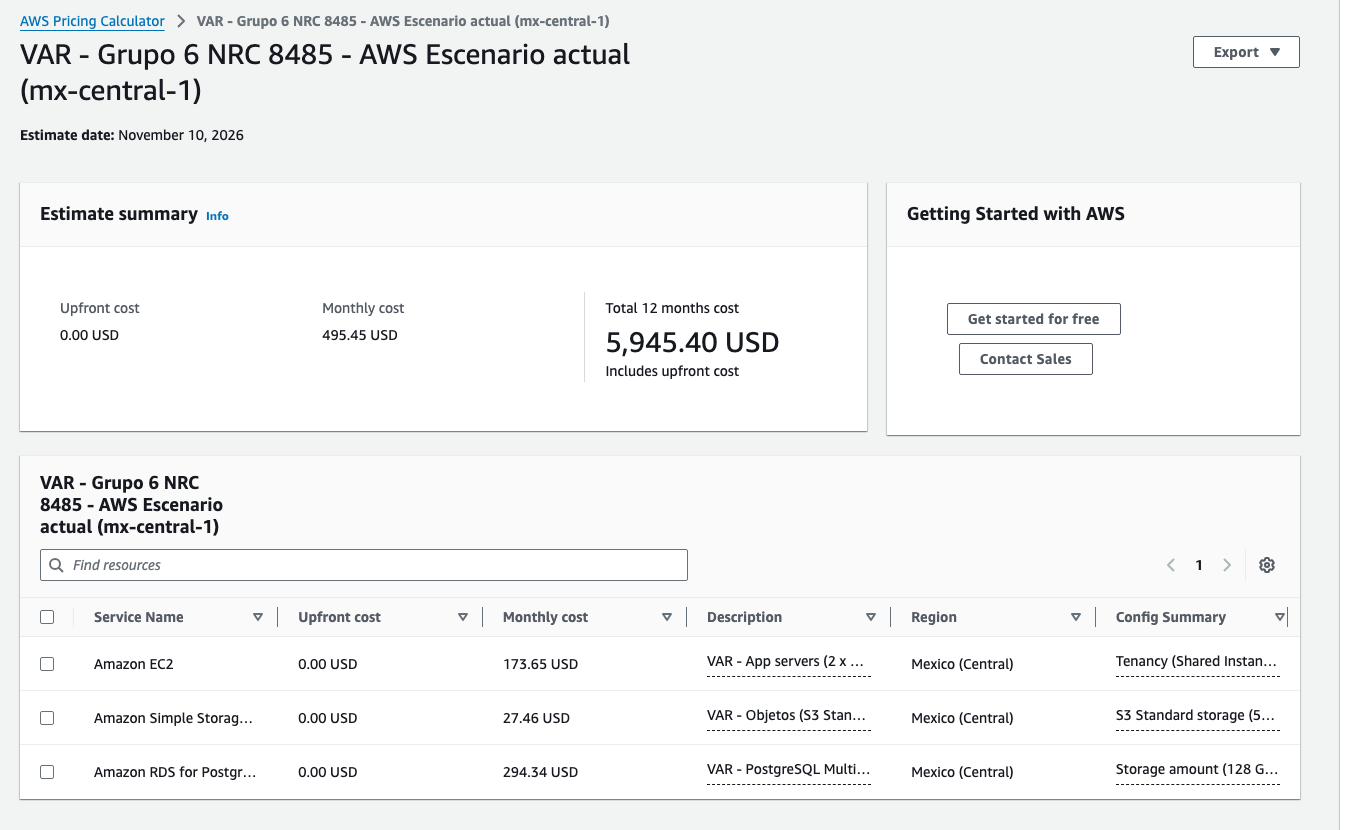
\includegraphics[width=0.92\linewidth]{figuras/calculadoras/aws-actual.png}\\[6pt]
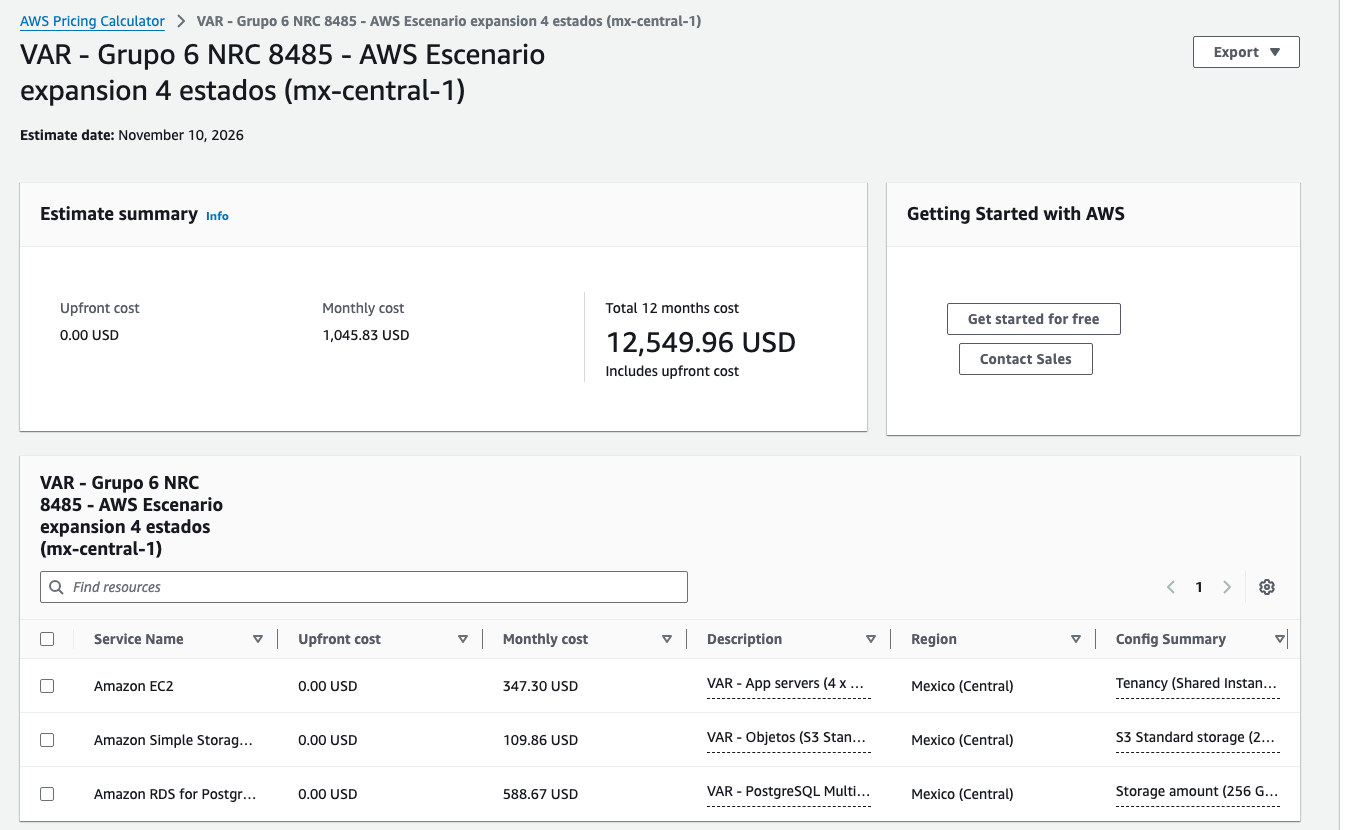
\includegraphics[width=0.92\linewidth]{figuras/calculadoras/aws-expansion.png}
\caption{AWS Pricing Calculator: escenario actual (arriba, 495,45 USD/mes) y de expansión (abajo, 1.045,83 USD/mes). Capturas del 10-11-2026.}\label{fig:calc-aws}
\end{figure}

\begin{figure}[H]
\centering
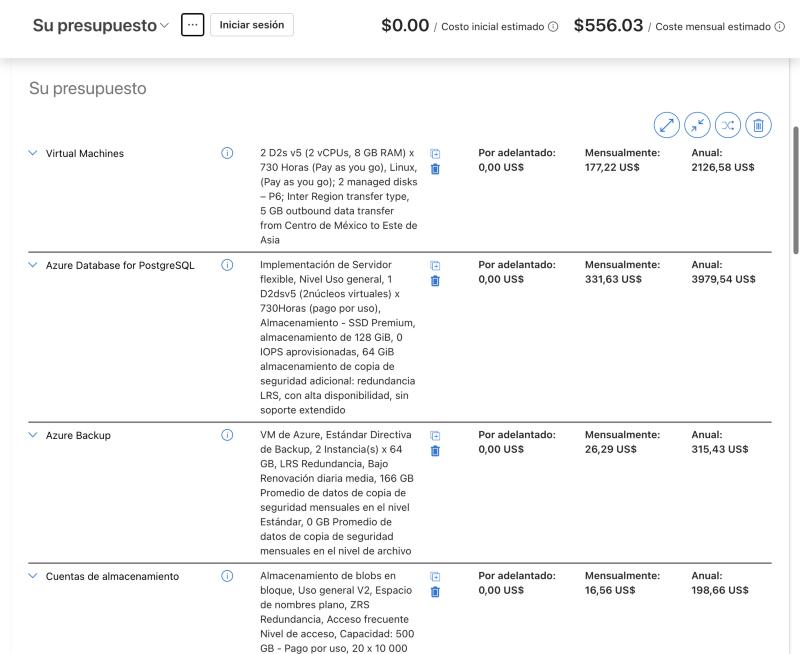
\includegraphics[width=0.74\linewidth]{figuras/calculadoras/azure-actual-1.jpg}\\[6pt]
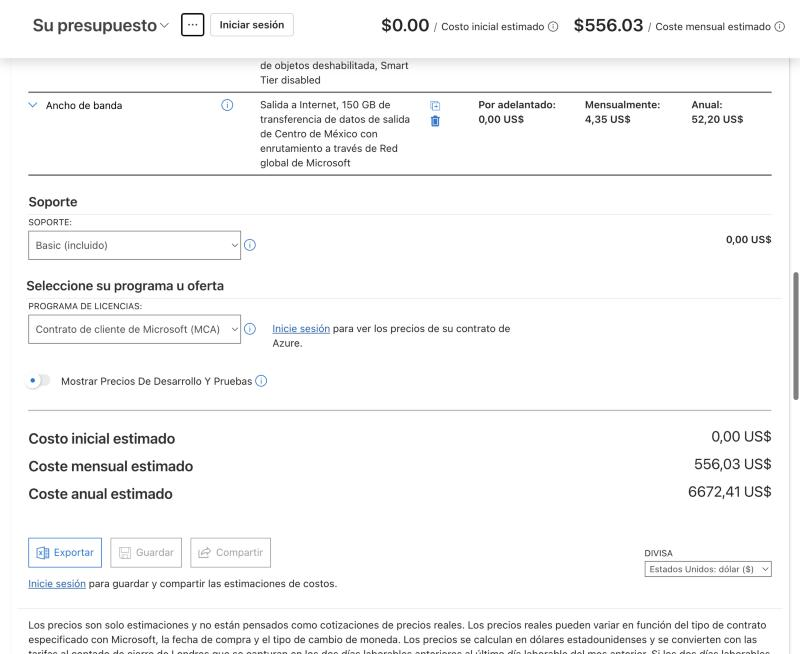
\includegraphics[width=0.74\linewidth]{figuras/calculadoras/azure-actual-3.jpg}
\caption{Azure Pricing Calculator, escenario actual: detalle por producto (arriba) y total de 556,03 USD/mes (abajo). Capturas del 10-11-2026.}\label{fig:calc-az-a}
\end{figure}

\begin{figure}[H]
\centering
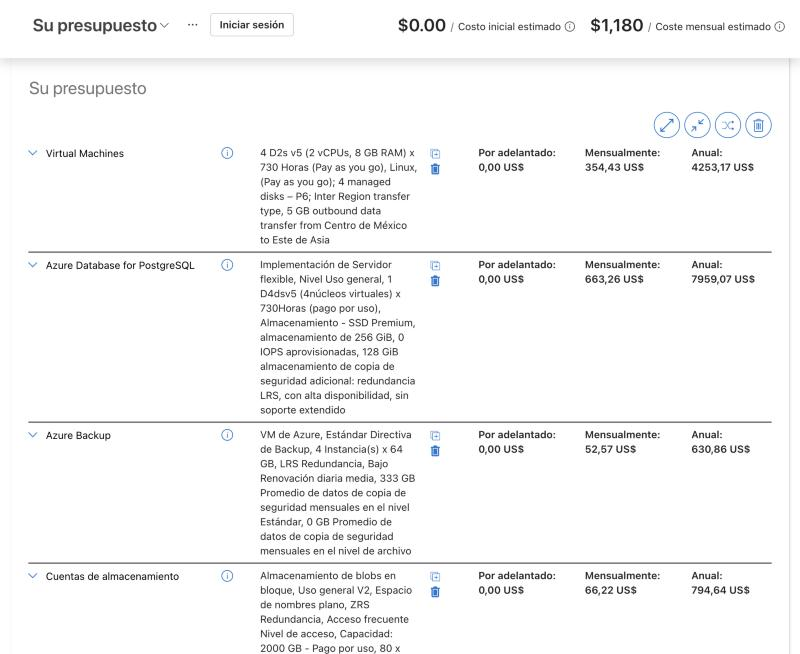
\includegraphics[width=0.74\linewidth]{figuras/calculadoras/azure-expansion-1.jpg}\\[6pt]
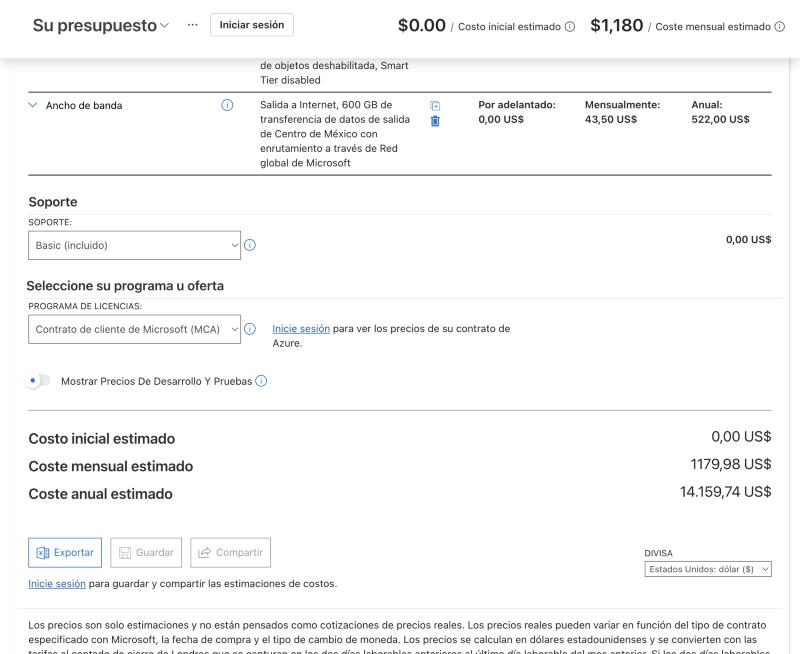
\includegraphics[width=0.74\linewidth]{figuras/calculadoras/azure-expansion-3.jpg}
\caption{Azure Pricing Calculator, escenario de expansión: detalle por producto (arriba) y total de 1.179,98 USD/mes (abajo). Capturas del 10-11-2026.}\label{fig:calc-az-b}
\end{figure}

\end{document}
